\documentclass[journal]{IEEEtran}
\usepackage[T1]{fontenc}
\usepackage{cite}
\usepackage{amsmath}
\usepackage{graphicx}
\graphicspath{{../}}
\usepackage{booktabs}
\usepackage{array}
\usepackage{url}
\usepackage[hidelinks]{hyperref}
\hypersetup{pdftitle={From MFCCs to Speech Foundation Models: Speaker-Independent Emotion Recognition on RAVDESS, Compared with Human Listeners}, pdfauthor={Muhammad Hassan Sohail}}
\makeatletter
\def\abstract{\normalfont\@IEEEabskeysecsize\bfseries\textit{\abstractname}:\ \relax\@IEEEgobbleleadPARNLSP}
\def\IEEEkeywords{\normalfont\@IEEEabskeysecsize\bfseries\textit{\IEEEkeywordsname}:\ \relax\@IEEEgobbleleadPARNLSP}
\makeatother

\begin{document}

\title{From MFCCs to Speech Foundation Models: Speaker-Independent Emotion Recognition on RAVDESS, Compared with Human Listeners}

\author{Muhammad~Hassan~Sohail%
\thanks{M. H. Sohail is with the University of Oulu, Oulu, Finland (e-mail: msohail24@student.oulu.fi). Research report for the course 521285S Affective Computing, autumn 2026. Code, predictions and logs: \url{https://github.com/hsn07pk/ravdess-speaker-independent-ser}.}}

\markboth{521285S Affective Computing, University of Oulu, 2026}{Sohail: Speaker-Independent Speech Emotion Recognition on RAVDESS}

\maketitle

\begin{abstract}
Published results for speech emotion recognition (SER) on the RAVDESS corpus range from about 72\% to above 90\%, partly because papers evaluate differently. We report one strictly speaker-independent evaluation: leave-one-speaker-out over all 24 actors, with the layer and the regularization chosen inside the training folds. Under the same linear probe we compare three handcrafted feature sets (mel-frequency cepstral coefficients with prosody, eGeMAPS and ComParE) with four frozen speech foundation models (WavLM, XLS-R, HuBERT and Whisper). The foundation models reach 77.8 to 81.9\% unweighted average recall (UAR) for eight emotions, against 63.6\% for the best handcrafted set, and logistic regression matches or beats a support vector machine and a random forest on every feature set. The most useful layers lie in the middle of the three wav2vec~2.0-type models and in the upper middle of Whisper; using the last layer costs up to 5.9 points. One end-to-end fine-tuning recipe for WavLM reaches only 73.2\%. A random split adds 7.2 to 13.4 points, per-speaker normalization 4.9 to 9.3, and choosing the layer on the test results up to 2.0. A public emotion model whose training data include RAVDESS reaches 79.9\% accuracy on seven options without any training on our side, so such models must be kept out of comparisons. We also compare the models with the human listeners clip by clip: on seven options the foundation models are more accurate than the average listener (79.6 to 83.6\% against 62.4\%), and they tend to find the same clips hard.
\end{abstract}

\begin{IEEEkeywords}
Evaluation protocol, human perception, RAVDESS, speaker independence, speech emotion recognition, speech foundation models.
\end{IEEEkeywords}

\section{Introduction}
\IEEEPARstart{S}{peech} carries emotion in how something is said: pitch, loudness, tempo and voice quality \cite{schuller2018ser,elayadi2011survey}. Speech emotion recognition (SER) tries to recover the speaker's emotional state from these cues, and it is one of the core problems of affective computing. Applications such as health monitoring or human-computer interaction meet new users all the time, so a system that only works for the voices it was trained on is of little use. The question that matters is how well SER works for a speaker it has never heard.

The Ryerson Audio-Visual Database of Emotional Speech and Song (RAVDESS) \cite{livingstone2018ravdess} is one of the most used corpora for this question. It has 24 professional actors who say the same two sentences in eight emotions, and it comes with ratings from human listeners for every clip. Published results for trained systems on its speech part range from about 72\% to above 90\% (Table~\ref{tab:literature}). Part of this spread comes from the evaluation rather than from better models. Some papers split the clips at random, so every test speaker is also in the training data. Some normalize each speaker with statistics of that speaker's own test recordings, which assumes many recordings of every new speaker. Some pick the best layer or epoch on the test data, and some use pretrained models whose training data included RAVDESS itself. Most of these are forms of data leakage \cite{kapoor2023leakage}. One study reports 91.7\% accuracy for Whisper features with a speaker-dependent split but 79.7\% with leave-one-speaker-out (LOSO) evaluation, although with different classifiers \cite{george2025whisper}.

At the same time the field has moved from handcrafted acoustic features to large pretrained speech encoders \cite{baevski2020wav2vec,hsu2021hubert,chen2022wavlm,babu2022xlsr,radford2023whisper}. Their layers carry different kinds of information \cite{pasad2021layerwise,li2022exploration}, and the last layer, which the EmoBox benchmark uses \cite{ma2024emobox}, is not always the best one for emotion.

This work asks four research questions (RQs) under one strict protocol, with unweighted average recall (UAR) as the main metric. RQ1: When the test speaker is unseen, how do handcrafted features with logistic regression (LR), support vector machines (SVMs) and random forests (RFs) compare with frozen speech foundation models, and with one that is fine-tuned end to end? RQ2: Which layers of these models carry the emotion information? RQ3: How much do common protocol choices, and pretrained models that may have seen RAVDESS, inflate the result? RQ4: Do the models fail on the same clips as the human listeners whose ratings come with RAVDESS? Our contributions are:
\begin{itemize}
\item \textbf{A layer-resolved, strictly speaker-independent comparison} (RQ1, RQ2) of four frozen foundation models, three handcrafted feature sets, three classifiers and an end-to-end fine-tuned WavLM: LOSO over all 24 actors, layer and regularization chosen inside the training folds, actor-level confidence intervals and paired tests.
\item \textbf{A measurement of protocol inflation inside one pipeline} (RQ3): random splits, per-speaker normalization and test-set layer selection, each applied to the same features and the same nested selection, for seven representations.
\item \textbf{A contamination example} (RQ3): a public emotion model whose training data include RAVDESS reaches the accuracy of our clean models without any training on our side.
\item \textbf{A per-clip comparison with human listeners} (RQ4), based on the ratings released with RAVDESS \cite{livingstone2018ravdess}.
\end{itemize}
What is new is the measurement, not the methods. We found no earlier RAVDESS study that compares several large foundation models layer by layer under nested LOSO, that measures several protocol shortcuts inside one pipeline (earlier work measured one at a time \cite{pepino2021wav2vec,george2025whisper}), or that compares model and listener errors clip by clip. The closest layer study \cite{li2022exploration} covered wav2vec~2.0 base checkpoints on four actor-disjoint folds. Section~\ref{sec:background} reviews acoustic features and classifiers for SER, from mel-frequency cepstral coefficients (MFCCs) with SVMs to speech foundation models, and Sections~\ref{sec:method} to~\ref{sec:discussion} present the experiment. Every result of ours was recomputed from the saved predictions by a separate script, and the code is public (see Reproducibility).

\section{Background and Related Work}
\label{sec:background}

\subsection{Handcrafted Features and Classical Classifiers}
Classical SER describes a clip with acoustic low-level descriptors computed over short frames and summarized by statistics (functionals) over the whole utterance \cite{elayadi2011survey,schuller2018ser}. MFCCs \cite{davis1980mfcc}, taken over from speech recognition, describe the spectral envelope. Prosodic features describe pitch (the fundamental frequency, F0), energy and timing. Pitch level and range separate high-arousal emotions such as anger and fear from sad or calm speech, but they say less about whether an emotion is positive or negative \cite{elayadi2011survey}. Standard feature sets combine both kinds: the extended Geneva Minimalistic Acoustic Parameter Set (eGeMAPS) has 88 parameters selected for their relevance in voice research \cite{eyben2016gemaps}, and the Computational Paralinguistics Challenge (ComParE) set has 6373 brute-force functionals \cite{schuller2016compare}; both are computed with openSMILE \cite{eyben2010opensmile}. The classifiers moved from Gaussian mixture models and hidden Markov models to SVMs \cite{cortes1995svm} and RFs \cite{breiman2001rf}, usually trained on one feature vector per utterance \cite{elayadi2011survey}.

\subsection{Deep Learning and Speech Foundation Models}
Deep networks first replaced the classifier and then the features. Recurrent networks with local attention learn which frames of an utterance matter \cite{mirsamadi2017attention}, and convolutional and recurrent networks learn from spectrograms and spectral features \cite{zhao2019cnnlstm,issa2020cnn} or from the raw waveform \cite{trigeorgis2016adieu}. These models still learn their representation from small labeled emotion corpora. The current step is to learn it instead by pretraining on large amounts of unlabeled or weakly labeled speech. Self-supervised models such as wav2vec~2.0 \cite{baevski2020wav2vec}, HuBERT \cite{hsu2021hubert} and WavLM \cite{chen2022wavlm} learn by predicting or contrasting masked parts of the signal. XLS-R \cite{babu2022xlsr} trains wav2vec~2.0 on 128 languages, and Whisper \cite{radford2023whisper} is an encoder-decoder trained with weak supervision to transcribe speech. We call such large pretrained encoders speech foundation models. Their hidden layers can be used frozen with a light classifier on top, as in the SUPERB \cite{yang2021superb} and EmoBox \cite{ma2024emobox} benchmarks, or fine-tuned end to end \cite{wagner2023dawn}. Layer-wise studies show that different layers hold different information and that the last layer is often not the best one for downstream tasks \cite{pasad2021layerwise}; for emotion, the middle layers of wav2vec~2.0 are among the best \cite{li2022exploration}. The emotion2vec model \cite{ma2024emotion2vec} is pretrained specifically for emotion.

\subsection{Speech Emotion Recognition on RAVDESS}
Table~\ref{tab:literature} lists representative results for the eight-class speech task. The protocols differ: speaker-dependent splits, LOSO, and fixed groups of four or five actors. Pepino et al.\ \cite{pepino2021wav2vec} showed that normalizing each speaker with its own statistics raises the results of wav2vec~2.0 features considerably, assuming that more recordings of the test speaker are available. Two more problems are less visible. First, the layer, the regularization or the epoch can be chosen on the test folds, which biases the estimate upwards \cite{varma2006bias,cawley2010overfitting}. Second, some public emotion models were trained on data that include RAVDESS, so they may have seen the test clips. For scale, the best zero-shot text-audio model we found, which is not trained on RAVDESS labels, reaches 46.0\% UAR on the eight classes \cite{yang2026clsp}.

RAVDESS also comes with ten ratings per clip from 247 listeners \cite{livingstone2018ravdess}. Each listener rated a pseudo-random set of 298 stimuli from the whole database, speech and song, after practice trials. For audio-only speech the mean proportion correct was 0.58 at normal and 0.67 at strong intensity.

\begin{table}[!t]
\centering
\caption{Published results on RAVDESS speech, eight classes. The protocols differ, so the numbers are not directly comparable. UAR: unweighted average recall (UA in \cite{ma2024emobox,yang2026clsp}); acc.: accuracy (WAR in \cite{sun2024hicmae}); LR: logistic regression; MLP: multilayer perceptron.}
\label{tab:literature}
\footnotesize
\setlength{\tabcolsep}{3pt}
\begin{tabular}{>{\raggedright\arraybackslash}p{2.0cm}>{\raggedright\arraybackslash}p{2.65cm}>{\raggedright\arraybackslash}p{1.75cm}r}
\toprule
Work & System & Protocol & Result \\
\midrule
George \& P \cite{george2025whisper} & Frozen Whisper-large + LR & LOSO & 79.3 UAR \\
 & Frozen Whisper-large + MLP & speaker-dependent & 91.7 acc. \\
Luna-Jim\'enez et al. \cite{lunajimenez2022proposal} & Fine-tuned XLSR-53 (English ASR checkpoint) & 5 folds by actor & 81.8 acc. \\
EmoBox \cite{ma2024emobox} & Frozen Whisper-large-v3, last layer & released split, 6 folds of 4 actors & 75.3 UAR \\
 & Frozen WavLM Large, last layer & same & 72.0 UAR \\
Sun et al. \cite{sun2024hicmae} & WavLM Base+, audio only & 6 folds by actor & 75.4 acc. \\
Yang et al. \cite{yang2026clsp} & CLSP, zero-shot & no training & 46.0 UAR \\
Livingstone \& Russo \cite{livingstone2018ravdess} & 247 listeners, audio only & listening test & 58 / 67 acc.$^{a}$ \\
\bottomrule
\multicolumn{4}{p{0.95\columnwidth}}{$^{a}$Mean proportion correct at normal / strong intensity; neutral and calm were accepted for each other, and ``none of these'' was an option.}
\end{tabular}
\end{table}


\section{Method}
\label{sec:method}

\subsection{Data}
We use the audio-only speech part of RAVDESS \cite{livingstone2018ravdess}: 1440 clips from 24 actors (12 female, 12 male) and eight emotions (neutral, calm, happy, sad, angry, fearful, disgust, surprised). Each actor says two sentences, each twice, for neutral at normal intensity and for the other seven emotions at normal and strong intensity, which gives 60 clips per actor; neutral has 96 clips and every other emotion 192. Leading and trailing silence is trimmed (30\,dB below the peak; the original clip is kept if the trimmed one is shorter than 0.1\,s). The audio is resampled to 16\,kHz, and to 22.05\,kHz for the librosa features.

\subsection{Representations}
\emph{Handcrafted.} (i) MFCC + prosody + spectral, 113 features computed with librosa \cite{mcfee2015librosa}: mean and standard deviation of 40 MFCCs; F0 statistics from pYIN \cite{mauch2014pyin} (65 to 500\,Hz) with the voiced fraction; root-mean-square (RMS) energy and zero-crossing rate; chroma, spectral contrast, centroid, bandwidth and roll-off. (ii) eGeMAPS v02 (88 functionals) and (iii) ComParE 2016 (6373 functionals), both from openSMILE \cite{eyben2010opensmile}.

\emph{Foundation models.} WavLM Large \cite{chen2022wavlm}, XLS-R 300M \cite{babu2022xlsr}, HuBERT Large \cite{hsu2021hubert} and the encoder of Whisper-large-v3 \cite{radford2023whisper}, all frozen and taken from the public checkpoints on the Hugging Face hub; we write WavLM, XLS-R, HuBERT and Whisper for them. For each clip we take every hidden layer (25 for the first three and 33 for Whisper, counting the input to the first Transformer layer as layer 0) and average it over time. Whisper pads every input to 30\,s, so we average only over the frames that cover the real clip. We also concatenate eGeMAPS with the WavLM layer chosen in each fold (1112 dimensions). The emotion2vec base model \cite{ma2024emotion2vec}, a base-size model whose pretraining data did not include RAVDESS, gives one 768-dimensional vector per clip.

\subsection{Classifiers and Nested Selection}
Every representation is classified with L2-regularized LR; we call LR on frozen, time-averaged features a linear probe. For the classifier comparison we also use an SVM with a radial basis function (RBF) kernel \cite{cortes1995svm} and an RF with 500 trees \cite{breiman2001rf}, all from scikit-learn \cite{pedregosa2011sklearn} with balanced class weights. LR and SVM features are standardized with statistics from the training actors only.

The outer loop is LOSO: each of the 24 actors is the test speaker once and is never used for training or for any choice. Inside each outer fold we run a 5-fold cross-validation, grouped by actor, on the 23 training actors. It chooses the layer and the regularization strength $C$ jointly, as the pair with the highest mean inner UAR; $C$ ranges from $10^{-4}$ to $10^{2}$ for LR and from $10^{-2}$ to $10^{3}$ for the SVM, one value per decade. The chosen model is refit on all 23 training actors and tested on the held-out actor. This nested design avoids the optimistic bias described in Section~\ref{sec:background}-C. The SVM uses the default kernel width, and its $C$ is chosen with hard predictions, while its reported predictions come from Platt-scaled probabilities; scoring the hard predictions instead changes the SVM results by $-0.3$ to $+2.0$ points. For WavLM the SVM and the RF use the layer chosen by the LR search, and the RF is not tuned, so this comparison favors LR.

\subsection{End-to-End Fine-Tuning}
We also fine-tune WavLM end to end on the same LOSO folds, using the course's computing project on the Roihu supercomputer of CSC, IT Center for Science, Finland. A learned weighted sum of all layers and a small head (a projection, mean pooling over time and a linear classifier) are trained together with the Transformer layers; the convolutional feature encoder stays frozen. We use AdamW with a learning rate of $3 \times 10^{-5}$ for the network and $10^{-3}$ for the head and the layer weights, weight decay 0.01, a linear schedule with 10\% warm-up, gradient clipping at 1.0, 10 epochs, batches of 8, class-weighted cross-entropy, bfloat16 mixed precision and the model's default time masking. In each fold the two actors with the next IDs after the test actor (one male, one female) are validation actors, used only to choose the epoch, and the model is trained on the other 21. The recipe was fixed before the run and not tuned, and it was run once, with one seed.

\subsection{Metrics and Statistics}
The primary metric is UAR, the mean recall over the eight classes, computed on the pooled out-of-fold predictions; we also report accuracy and macro-F1. Since every actor has the same number of clips per class, pooled UAR equals the mean of the 24 per-actor UARs. Confidence intervals come from an actor-level bootstrap with 10\,000 resamples \cite{efron1993bootstrap}. Systems are compared with the paired Wilcoxon signed-rank test over the 24 per-actor UARs \cite{wilcoxon1945,demsar2006statistical}, with Holm correction \cite{holm1979} over the 23 comparisons of our main test family; the fine-tuning test and the female-versus-male Mann-Whitney U tests are reported without correction. Because the folds share most of their training actors, these tests and intervals are approximate \cite{nadeau2003inference}. As a sanity check we rerun the whole nested pipeline on WavLM with the labels permuted within each actor, with three seeds \cite{ojala2010permutation}.

\subsection{Further Analyses}
\emph{Protocol inflation.} We rerun the nested pipeline with (a) a random stratified 5-fold split, so every test speaker also appears in training, and for most test clips the other recording of the same sentence, emotion and intensity does too; and (b) LOSO after normalizing each actor's features with that actor's own mean and standard deviation, which uses the test speaker's unlabeled audio. We also report (c) the best single layer picked on the test results, as a layer study without nested selection would.

\emph{EmoBox anchor.} To compare with published numbers we evaluate the last layer on the six released EmoBox folds of four actors \cite{ma2024emobox}.

\emph{Contamination.} The emotion2vec+ large model builds on a model that was fine-tuned on the EmoBox data, which include RAVDESS \cite{emotion2vecplus}. We score it zero-shot with its own head on the seven options defined below, and also as a LOSO linear probe.

\emph{Human comparison.} The listeners chose among eight emotions and ``None of these are correct'', and neutral and calm were accepted for each other \cite{livingstone2018ravdess}. We score the models the same way: the neutral and calm probabilities are summed, which gives seven options. Per clip, the human score is the share of the ten ratings that name the intended emotion; its mean over clips is the listeners' mean proportion correct.

\section{Results}
\label{sec:results}

\begin{table*}[!t]
\centering
\caption{Main results: leave-one-speaker-out over 24 actors, eight classes. Every representation is classified with LR (linear probe), except the fine-tuned WavLM, which is trained end to end with the epoch chosen on two validation actors. Layer and $C$ are chosen inside each training fold. Layers chosen: range over the 24 folds (most frequent layer: number of folds). CI: 95\% actor-level bootstrap.}
\label{tab:main}
\begin{tabular}{lccccc}
\toprule
Representation & Dim. & Layers chosen & UAR \% [95\% CI] & Acc. \% & Macro-F1 \% \\
\midrule
XLS-R 300M & 1024 & 8--15 (10: 12) & 81.9 [77.8, 85.9] & 81.7 & 81.4 \\
WavLM Large & 1024 & 9--11 (10: 13) & 81.3 [77.1, 85.2] & 81.2 & 81.0 \\
Whisper-large-v3 enc. & 1280 & 20--26 (22: 6) & 80.2 [75.8, 84.3] & 80.3 & 79.7 \\
HuBERT Large & 1024 & 11--15 (14: 10) & 77.8 [72.5, 82.6] & 77.6 & 77.4 \\
WavLM Large + eGeMAPS & 1112 & as WavLM Large & 81.6 [77.5, 85.4] & 81.7 & 81.4 \\
WavLM Large, fine-tuned & 1024 & weighted sum & 73.2 [66.5, 79.0] & 72.4 & 72.0 \\
emotion2vec base & 768 & utterance vector & 66.7 [62.3, 70.8] & 66.3 & 66.2 \\
\midrule
ComParE 2016 & 6373 & n/a & 63.6 [59.0, 68.4] & 63.4 & 62.8 \\
eGeMAPS v02 & 88 & n/a & 53.1 [49.5, 56.4] & 52.7 & 52.1 \\
MFCC + prosody + spectral & 113 & n/a & 50.5 [45.6, 55.5] & 50.8 & 49.7 \\
\midrule
WavLM Large, labels permuted (3 seeds) & 1024 & per fold & 13.4 (range 12.5--13.9) & n/a & n/a \\
Chance & & & 12.5 & n/a & n/a \\
\bottomrule
\end{tabular}
\end{table*}


\begin{figure*}[!t]
\centering
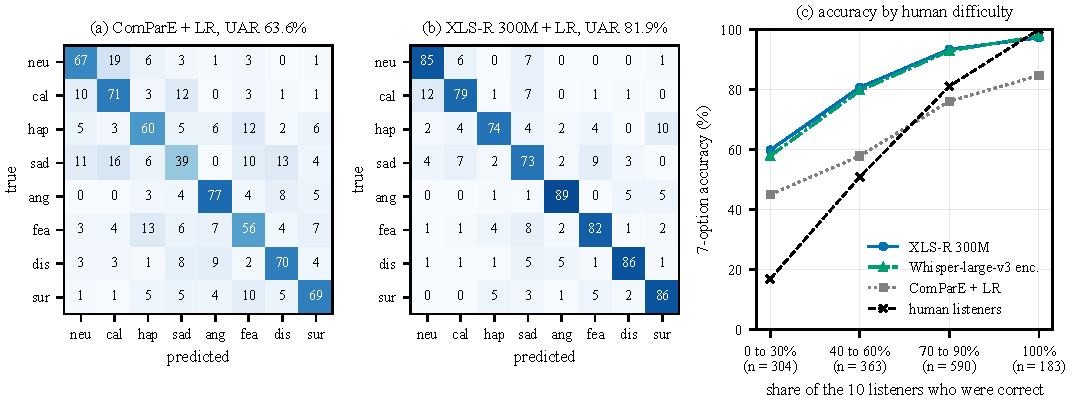
\includegraphics[width=\textwidth]{figures/confusions_human.pdf}
\caption{(a, b) Row-normalized confusion matrices (\%) of ComParE + LR and XLS-R 300M + LR, eight classes, LOSO (neu: neutral, cal: calm, hap: happy, ang: angry, fea: fearful, dis: disgust, sur: surprised). (c) Seven-option accuracy against the share of the ten listeners who were correct on a clip; $n$ is the number of clips in each group. The listener curve is the mean share of correct ratings in each group, so it rises by construction.}
\label{fig:conf}
\end{figure*}

\subsection{Feature Sets and Classifiers (RQ1)}
Table~\ref{tab:main} gives the main results. The four foundation models reach 77.8 to 81.9\% UAR, 14.2 to 18.3 points above the best handcrafted set, ComParE (63.6\%). Each of them beats ComParE for 22 or 23 of the 24 actors ($p_{\text{Holm}} \le 0.0014$). The differences among the foundation models are not significant after correction; the largest, WavLM and XLS-R over HuBERT (+3.5 and +4.1 points), both have $p_{\text{Holm}} = 0.075$. XLS-R has the highest point estimate (81.9\%), above the best strict LOSO result we found, 79.3\% for frozen Whisper-large features \cite{george2025whisper}, but within our confidence interval; our own Whisper probe (80.2\%) is close to that published number. Adding eGeMAPS to WavLM changes UAR by only +0.3 points (not significant), so in this early fusion the handcrafted descriptors add little. The emotion2vec base model, a base-size model used as one utterance vector, reaches 66.7\%, not significantly different from ComParE.

Among the handcrafted sets, ComParE beats eGeMAPS by 10.5 points and the MFCC + prosody + spectral set by 13.1 ($p_{\text{Holm}} \le 0.005$); eGeMAPS and the MFCC set do not differ significantly. LR is the best or equal-best classifier for every feature set (Table~\ref{tab:classifiers}). The SVM is within 0.3 points of LR on WavLM and on the MFCC set but 1.9 and 4.1 points lower on eGeMAPS and ComParE (not tested), and the RF is worse for every feature set, by 1.8 to 11.3 points; its drop is significant on WavLM ($-5.8$ points, $p_{\text{Holm}} = 0.018$).

Two checks support the pipeline. With the labels permuted within each actor, WavLM gives 13.4\% (mean of three seeds), close to the 12.5\% chance level. On the released EmoBox folds our last-layer probe gives 75.3\% for WavLM, 70.8\% for HuBERT and 76.5\% for Whisper, 0.8 to 3.3 points above the 72.0, 70.0 and 75.3\% reported by EmoBox \cite{ma2024emobox}, which uses a small neural head instead of LR.

Fig.~\ref{fig:conf}(a,b) shows the confusions. ComParE hears neutral as calm (19\%), sad as calm and as disgust (16\% and 13\%) and happy as fearful (12\%), and it recognizes only 39\% of the sad clips. XLS-R keeps at least 73\% recall for every emotion; its largest confusions are calm heard as neutral (12\%), happy as surprised (10\%) and sad as fearful (9\%).

\begin{table}[!t]
\centering
\caption{UAR (\%) of three classifiers on the same nested protocol. For WavLM Large the SVM and the RF use the layer chosen per fold by the LR search; $C$ is re-tuned for the SVM, and the RF (500 trees) is not tuned.}
\label{tab:classifiers}
\begin{tabular}{lccc}
\toprule
Features & LR & SVM (RBF) & RF \\
\midrule
MFCC + prosody + spectral & 50.5 & 50.5 & 48.1 \\
eGeMAPS v02 & 53.1 & 51.2 & 51.2 \\
ComParE 2016 & 63.6 & 59.5 & 52.3 \\
WavLM Large & 81.3 & 81.0 & 75.5 \\
\bottomrule
\end{tabular}
\end{table}


\subsection{End-to-End Fine-Tuning (RQ1)}
Fine-tuning WavLM end to end gives 73.2\% UAR (Table~\ref{tab:main}), 8.1 points below the linear probe on the same model. It is worse for 18 of the 24 actors, better for 3 and equal for 3 ($p = 2.9 \times 10^{-4}$, one planned test outside the Holm family). The loss is uneven: the median actor loses 4.7 points, but the five worst actors lose 17.2 to 35.9 points each. In two folds (test actors 7 and 13) training did not converge: the training loss was still 0.93 and 0.94 after ten epochs, against 0.01 to 0.11 in the other folds, and these folds give 43.8 and 25.0\% UAR. The per-actor standard deviation is 16.3 points, against 10.4 for the linear probe. The comparison is not fully matched, since the fine-tuned model trains on 21 actors and picks its epoch on two, while the probe uses all 23 with grouped cross-validation. Luna-Jim\'enez et al.\ report 81.8\% accuracy for a fine-tuned XLSR-53 with five folds by actor \cite{lunajimenez2022proposal}, so a different or tuned recipe can do better. The 24 folds used 1.26 GPU hours on NVIDIA GH200 GPUs.

\begin{figure}[!t]
\centering
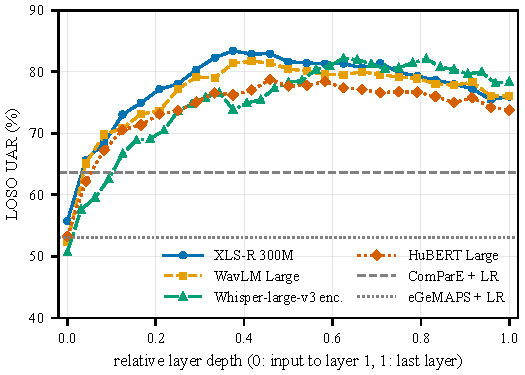
\includegraphics[width=\columnwidth]{figures/layer_curves.pdf}
\caption{LOSO UAR (eight classes) of LR on each single layer of the four frozen models, against relative depth (0: input to the first Transformer layer, 1: last layer); $C$ is chosen inside the training folds. Grey lines: ComParE + LR and eGeMAPS + LR. Chance is 12.5\%.}
\label{fig:layers}
\end{figure}

\subsection{Where the Emotion Information Sits (RQ2)}
Fig.~\ref{fig:layers} shows the UAR of each layer. For XLS-R, WavLM and HuBERT, UAR rises quickly over the first third of the network, peaks in the middle (layers 9 to 11 of 24) and falls towards the last layer. Whisper rises more slowly and peaks in the upper middle (layer 20 of 32). The nested selection agrees with this: it picked layers 8 to 15 for the three wav2vec~2.0-type models and 20 to 26 for Whisper. Using the last layer instead costs 5.3 points for WavLM and 5.9 for XLS-R ($p_{\text{Holm}} = 0.014$ and $0.015$), and 4.0 for HuBERT and 1.8 for Whisper (not significant after correction). Averaging all layers is a reasonable alternative (77.5 to 81.2\%). It is below the nested choice for the three wav2vec~2.0-type models and 0.8 points above it for Whisper.

\begin{table}[!t]
\centering
\caption{Protocol inflation, UAR (\%). Change against the strict nested LOSO result in parentheses. The random 5-fold split and the per-speaker normalization (Spk. norm.) repeat the full nested selection; the last column picks the best layer on the test results. Whisper-L-v3: Whisper-large-v3 encoder; MFCC + pros. + spec.: MFCC + prosody + spectral.}
\label{tab:inflation}
\setlength{\tabcolsep}{2pt}
\begin{tabular}{lcccc}
\toprule
Representation & LOSO & Random 5-fold & Spk. norm. & Layer on test \\
\midrule
XLS-R 300M & 81.9 & 89.4 (+7.5) & 86.8 (+4.9) & 83.4 (+1.5) \\
WavLM Large & 81.3 & 91.7 (+10.4) & 87.3 (+6.0) & 81.7 (+0.4) \\
Whisper-L-v3 & 80.2 & 90.4 (+10.2) & 89.1 (+8.9) & 82.2 (+2.0) \\
HuBERT Large & 77.8 & 89.1 (+11.3) & 85.1 (+7.3) & 78.7 (+0.9) \\
ComParE 2016 & 63.6 & 73.6 (+10.0) & 72.2 (+8.6) & n/a \\
eGeMAPS v02 & 53.1 & 60.3 (+7.2) & 62.2 (+9.1) & n/a \\
MFCC + pros. + spec. & 50.5 & 63.9 (+13.4) & 59.8 (+9.3) & n/a \\
\bottomrule
\end{tabular}
\end{table}


\subsection{Protocol Inflation and Contamination (RQ3)}
Table~\ref{tab:inflation} shows what happens when the same features and the same nested selection are evaluated with weaker protocols. A random 5-fold split, where every test speaker is also in training, adds 7.5 to 11.3 points for the foundation models and 7.2 to 13.4 for the handcrafted sets; WavLM goes from 81.3 to 91.7\%. Normalizing each speaker with its own statistics adds 4.9 to 9.3 points without any labeled data from the test speaker. Every RAVDESS actor has the same balanced set of emotions, so these statistics are unusually favorable, and the gain is likely larger than it would be with real users. Picking the best layer on the test results adds up to 2.0 points. The random-split gains are of the same order as the difference between ComParE and eGeMAPS (10.5 points), and both the random-split and the speaker-normalization gains are larger than every difference among the foundation models (at most 4.1 points), so results from different protocols should not be compared directly.

The contaminated emotion2vec+ large model reaches 79.9\% accuracy (79.3\% UAR) on the seven options without any training on our side, within the range of our clean models on the same options (79.6 to 83.6\%, Table~\ref{tab:human}), and 77.5\% UAR as a LOSO probe, just below the four clean frozen models. Its zero-shot score is far above that of the best zero-shot text-audio model (46.0\% UAR \cite{yang2026clsp}), although that model uses eight classes and is not directly comparable. These numbers cannot tell whether the model recalls clips it has seen or transfers genuinely, and that is exactly why such a model must not be compared with clean ones.

\begin{table}[!t]
\centering
\caption{Listeners and models on the same 1440 clips, seven options (neutral and calm merged). For the listeners: mean proportion correct. $\rho$: Spearman correlation between the share of correct ratings per clip and the model's probability for the true emotion. Hard clips: at most four of the ten listeners correct ($n=414$).}
\label{tab:human}
\begin{tabular}{lccc}
\toprule
System & Acc. \% & $\rho$ & Acc. on hard clips \% \\
\midrule
Human listeners & 62.4 & n/a & n/a \\
XLS-R 300M & 83.6 & 0.47 & 63.5 \\
WavLM Large & 82.9 & 0.49 & 63.3 \\
Whisper-large-v3 enc. & 82.8 & 0.45 & 62.3 \\
HuBERT Large & 79.6 & 0.42 & 59.4 \\
ComParE 2016 & 66.0 & 0.37 & 46.1 \\
eGeMAPS v02 & 55.3 & 0.42 & 33.1 \\
MFCC + prosody + spectral & 56.2 & 0.41 & 33.6 \\
\bottomrule
\end{tabular}
\end{table}


\subsection{Humans and Machines (RQ4)}
The listeners named the intended emotion in 62.4\% of their ratings: 58.0\% at normal and 67.4\% at strong intensity, consistent with Table~2 of \cite{livingstone2018ravdess}. Scored on the same seven options, the four foundation models reach 79.6 to 83.6\% (Table~\ref{tab:human}). This does not mean that the models hear emotion better than people. The listeners rated pseudo-random sets of stimuli after only a few practice trials, while the models learned from 1380 labeled clips of 23 other actors saying the same two sentences, and the listeners could also answer ``none of these''.

The models do, however, tend to find the same clips hard. The model's probability for the true emotion correlates with the share of correct ratings per clip ($\rho = 0.42$ to $0.49$ for the foundation models and 0.37 to 0.42 for the handcrafted sets); part of this correlation comes from emotions and intensities that are hard for both. Fig.~\ref{fig:conf}(c) shows that the accuracy of XLS-R rises from 59.9\% on the 304 clips that at most three of the ten listeners got right to 97.3\% on the 183 clips that all ten got right. On the 414 hard clips, which at most four listeners got right, the foundation models are still correct 59.4 to 63.5\% of the time, against 33.1 to 46.1\% for the handcrafted sets. The listeners find happy speech hardest (36.6\%), where XLS-R reaches 74.0\%; both do best on neutral/calm (81.7 and 91.7\%). Strong intensity helps both: the listeners go from 58.0 to 67.4\% and XLS-R from 81.2 to 86.3\% seven-option accuracy.

Per-actor UAR is 8.6 to 12.4 points higher for the 12 female than for the 12 male actors for all four foundation models, significant only for HuBERT and only without correction (Mann-Whitney U, $p = 0.022$). The listeners show the same direction: their mean proportion correct is 66.1\% for the female and 58.6\% for the male actors ($p = 0.035$), so the gap may come from the portrayals rather than from the models.

\section{Discussion}
\label{sec:discussion}
\emph{RQ1.} Under a protocol that keeps the test speaker unseen, frozen foundation models with a linear probe are 14 to 18 points better than the best handcrafted set, and three of the four (80.2 to 81.9\%) are on par with or slightly above the best strict LOSO result we found in the literature. Among the handcrafted features, the large brute-force ComParE set clearly beats eGeMAPS and the MFCC + prosody + spectral set, and LR is never worse than the SVM or the RF, although our comparison favors LR. The largest ComParE confusions are between emotions of similar arousal (neutral heard as calm, sad as calm, happy as fearful), as expected if prosodic cues carry arousal better than valence \cite{elayadi2011survey}. Our single fine-tuning recipe was 8.1 points worse than the linear probe and did not converge in two folds. With 21 training actors it was fragile, which does not show that fine-tuning cannot match the probe \cite{wagner2023dawn,lunajimenez2022proposal}. In our setting the linear probe was both the stronger and the cheaper choice, since it needs no GPU training.

\emph{RQ2.} The middle layers carry the most emotion information, so a last-layer probe, as in EmoBox, underestimates WavLM and XLS-R by 5 to 6 points. Nested layer selection, or the average of all layers, avoids this.

\emph{RQ3.} Part of the higher numbers reported for RAVDESS may come from the protocol rather than from better models: the random-split and speaker-normalization gains in Table~\ref{tab:inflation} are larger than the differences among the four foundation models. A model that may have seen RAVDESS reaches the accuracy of the clean models without any training, so the training data of a pretrained model must be checked before it is compared.

\emph{RQ4.} Both the foundation models and the handcrafted sets track human difficulty, so the clips that listeners find hard tend to be hard for every representation.

\emph{Limitations.} RAVDESS is acted, read speech of two fixed sentences by 24 North American actors, so LOSO here is speaker-independent but not text-independent, and results on spontaneous speech, other languages or noisy recordings are likely to be lower; we did not test across corpora. With 24 actors the 95\% confidence intervals are about 7 to 10 points wide and the tests are approximate, so only large differences are clear. We fine-tuned only WavLM, with one recipe and one seed. The speaker-normalization gain depends on the balanced design of RAVDESS. We cannot show that the emotion2vec+ model memorized RAVDESS, only that it may have seen it. The training audio of Whisper is not public, so we cannot rule out that it contains RAVDESS clips, although it was trained without emotion labels. The human score is the mean accuracy of single ratings, not the accuracy of a listener panel.

\section{Conclusion}
Under one strict speaker-independent protocol on RAVDESS, frozen speech foundation models with a linear probe reach 77.8 to 81.9\% UAR for eight emotions, 14 to 18 points above the best handcrafted features. Their best layers lie in the middle of the network for the wav2vec~2.0-type models and in the upper middle for Whisper. One end-to-end fine-tuning recipe for WavLM was 8.1 points worse than its linear probe. On the same pipeline, a random split would have added up to 13.4 points, speaker normalization up to 9.3 and test-set layer selection up to 2.0, and a public model that may have seen RAVDESS matches the clean models without any training. We recommend LOSO with nested selection, UAR with actor-level confidence intervals, layer selection inside the training folds, and a check of what data a pretrained model has seen.

\section*{Acknowledgment}
We thank CSC, IT Center for Science, Finland, for computing time on the Roihu supercomputer.

\section*{Reproducibility}
The code, the out-of-fold predictions of every system, the logs and the scripts that produce every table and figure are available at \url{https://github.com/hsn07pk/ravdess-speaker-independent-ser}. Every reported result of ours was recomputed from the saved predictions with code independent of the evaluation pipeline (1640 checks, all passed).

\bibliographystyle{IEEEtran}
\bibliography{refs}

\end{document}
